%%%%%%%%%%%%%%%%%%%%%%%%%%%%%%%%%%%%%%%%%%%%%%%%%%%%%%%%%%%%%%%%%%%%%%%%%%%%%%%%
%2345678901234567890123456789012345678901234567890123456789012345678901234567890
%        1         2         3         4         5         6         7         8
%% main.tex
%% V1.0
%% 2017/02/22
%% by Francisco Maria Calisto
%% based on a template created by Rob Oakes
%%%%%%%%%%%%%%%%%%%%%%%%%%%%%%%%%%%%%%%%%%%%%%%%%%%%%%%%%%%%%%%%%%%%%%%%%%%%%%%%

\documentclass[a4paper,12pt]{texDoc}
% --> Please Choose the MAIN LANGUAGE for the document in package BABEL
% --> by replacing "main=" in language name selector. Default is "main=english"
\usepackage[main=english,portuguese]{babel} % Defines Main language
\usepackage[utf8]{inputenc}
\usepackage{iflang}
\usepackage{ifthen}
\usepackage{parskip}
\setlength{\parindent}{15pt}
\logo{
\includegraphics[width=0.3\textwidth]{IST_A_RGB_POS.png}} % Logo

%%%%%%%%%%%%%%%%%%%%%%%%%%%%%%%%%%%%%%%%%%%%%%%%%%%%%%%%%%%%%%%%%%%%%%%%%%%%%%%%
%	MEMO INFORMATION --> Write your info in the following tags.
%%%%%%%%%%%%%%%%%%%%%%%%%%%%%%%%%%%%%%%%%%%%%%%%%%%%%%%%%%%%%%%%%%%%%%%%%%%%%%%%

\docfrom{Francisco Maria Calisto} % Sender(s) Name
\docid{ist170916} % Student ID
\doccourse{AE 2016/2017} % Course Name, or abbreviated acronym
\docsubject{Problem Sheet \# 1 - Study} % Subject
\docdate{\today} % Date, -> set to \today for automatically print todays date

%%%%%%%%%%%%%%%%%%%%%%%%%%%%%%%%%%%%%%%%%%%%%%%%%%%%%%%%%%%%%%%%%%%%%%%%%%%%%%%%

\begin{document}
\maketitle % Print the doc header information

%%%%%%%%%%%%%%%%%%%%%%%%%%%%%%%%%%%%%%%%%%%%%%%%%%%%%%%%%%%%%%%%%%%%%%%%%%%%%%%%
%	LETTER CONTENT --> Your content is written here
%%%%%%%%%%%%%%%%%%%%%%%%%%%%%%%%%%%%%%%%%%%%%%%%%%%%%%%%%%%%%%%%%%%%%%%%%%%%%%%%

\section*{Question 1}

\subsection*{Answer}

R: b)

Why do I believe that I am correct?

b) The defined concepts and description of a system architecture and requirements for determine whether the description of an architecture conforms with are:

- Structural/Behavioural: behavioural concepts are the Assign to structural elements (assets) To indicate who or what offers certain behaviour.

- External/Internal: external or internal view of "systems".

- Individual/ Collective-Distinction: between behaviour executed by individual structural elements and collective behaviour performed by a collaboration of multiple structural elements.

\subsection*{Why the others are wrong?}

a) A representative enterprise architecture should be defined \cite{eaFundamentals} by three layers:

- Business: it offers services to customers through products, where the services are realized by business processes that use the informational entities of the organization and run by business actors.

- Application: supports the level of business with application services realized in application components.

- Technological: provides infrastructure services, like processing, storage and communication, to the application layer and it is where also the services are realized by software, machines and computer devices.

\begin{center}
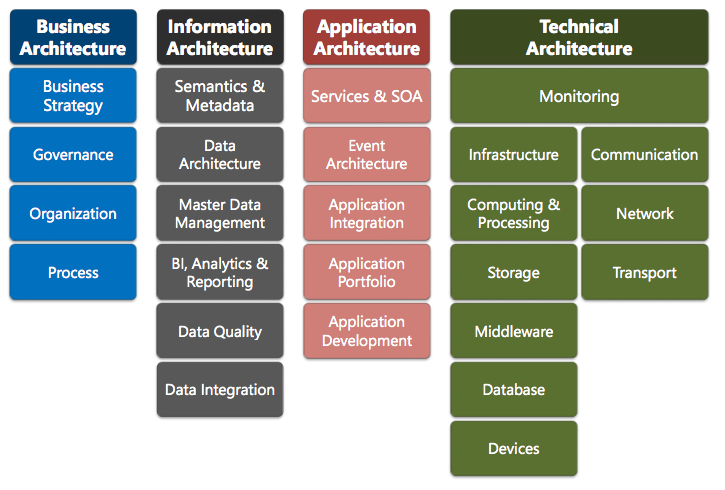
\includegraphics[width=0.75\textwidth]{concepts.png}
\end{center}

c) To establish concepts and methods, to identify and specify views and perspectives on the architecture, it may be relevant to distinguish between architecture principles that are relevant to:

- All employees of the organization.

- Employees of a specific part of the organization (business unit).

- Principles that are only relevant to employees in a specific role (e.g. software developers).

d) The standard focuses on the concepts of business process and stakeholder are:

\begin{center}
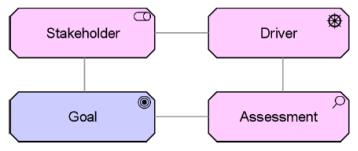
\includegraphics[width=0.75\textwidth]{stakeholders.png}
\end{center}

Since the stakeholder viewpoint focuses on modeling the stakeholders, drivers, the assessments of these drivers, and the initial goals to address these drivers and assessments.

\section*{Question 2}


%%%%%%%%%%%%%%%%%%%%%%%%%%%%%%%%%%%%%%%%%%%%%%%%%%%%%%%%%%%%%%%%%%%%%%%%%%%%%%%%
%	DOCUMENT BIBLIOGRAPHY --> Your bibliography is written here
%%%%%%%%%%%%%%%%%%%%%%%%%%%%%%%%%%%%%%%%%%%%%%%%%%%%%%%%%%%%%%%%%%%%%%%%%%%%%%%%

\begin{thebibliography}{9}
\bibitem{eaFundamentals}  Enterprise Architecture Fundamentals. Available from World Wide Web: (AE\_fundamentals\_Fev\_2017\_v0\_8.pdf).
\end{thebibliography}

%%%%%%%%%%%%%%%%%%%%%%%%%%%%%%%%%%%%%%%%%%%%%%%%%%%%%%%%%%%%%%%%%%%%%%%%%%%%%%%%
\end{document}